% HDC-RWKV (nb12c) — FULL EXPANDED architecture poster (v2: spacing fixed).
%
% Companion to:
%   - architecture_hdc_rwkv.tex       (compact block diagram)
%   - architecture_walkthrough.tex    (worked numerical example)
%
% This file expands every block from the compact diagram to show its
% internal structure. v2 increases horizontal/vertical padding and removes
% the Block 2 overdraw hack from v1.
%
% Compile:  pdflatex architecture_hdc_rwkv_expanded.tex

\documentclass[tikz,border=14pt]{standalone}
\usepackage{tikz}
\usepackage{amsmath,amssymb}
\usepackage{xcolor}
\usetikzlibrary{positioning,arrows.meta,calc,fit,backgrounds,shapes.geometric,
                shapes.misc,decorations.pathreplacing,decorations.markings,matrix}

% Math macros
\newcommand{\bV}{\mathbf{V}}
\newcommand{\bP}{\mathbf{P}}
\newcommand{\bm}{\mathbf{m}}
\newcommand{\bh}{\mathbf{h}}
\newcommand{\bs}{\mathbf{s}}
\newcommand{\bipset}{\{-1,+1\}}

% ============================================================ colour palette
\definecolor{cBipolar}{HTML}{2C5282}
\definecolor{cBipolarLite}{HTML}{EBF4FF}
\definecolor{cCont}{HTML}{B7791F}
\definecolor{cContLite}{HTML}{FFF8E6}
\definecolor{cOp}{HTML}{2D3748}
\definecolor{cSampler}{HTML}{6B46C1}
\definecolor{cSamplerLite}{HTML}{F3EBFF}
\definecolor{cAux}{HTML}{276749}
\definecolor{cAuxLite}{HTML}{F0FFF4}
\definecolor{cArrow}{HTML}{1A202C}
\definecolor{cPanelBg}{HTML}{FAFBFC}
\definecolor{cPanelBorder}{HTML}{CBD5E0}

% ================================================================== styles
\tikzset{
  block/.style={draw=cPanelBorder, fill=cPanelBg, thick, rounded corners=6pt,
                inner sep=8pt},
  blockTitle/.style={font=\bfseries\large, anchor=north west,
                     inner sep=4pt, xshift=4pt, yshift=-4pt},
  cellPos/.style={draw=cBipolar!50, fill=cBipolarLite, font=\scriptsize,
                  minimum width=7mm, minimum height=6mm, inner sep=0pt},
  cellNeg/.style={draw=cBipolar!50, fill=cBipolar!18, font=\scriptsize,
                  minimum width=7mm, minimum height=6mm, inner sep=0pt},
  cellCont/.style={draw=cCont!60, fill=cContLite, font=\scriptsize,
                   minimum width=11mm, minimum height=6mm, inner sep=0pt},
  cellPlain/.style={draw=black!30, fill=white, font=\scriptsize,
                    minimum width=7mm, minimum height=6mm, inner sep=0pt},
  op/.style={draw=cOp, fill=white, thick, circle, inner sep=1.4pt,
             font=\small, minimum size=6mm},
  flow/.style={-{Stealth[length=2mm]}, thick, draw=cArrow},
  flowSm/.style={-{Stealth[length=1.6mm]}, semithick, draw=cArrow!85},
  recur/.style={-{Stealth[length=2mm]}, thick, draw=cCont!80!black, dashed},
  lbl/.style={font=\scriptsize\itshape, text=black!65, align=center},
  matlbl/.style={font=\scriptsize, text=cBipolar!85!black, align=center},
  idx/.style={font=\scriptsize\ttfamily, text=black!55},
  eqn/.style={font=\small},
  panel/.style={draw=cPanelBorder, fill=cPanelBg, thick, rounded corners=4pt,
                inner sep=6pt},
}

\newcommand{\bipRowAt}[4]{% #1 prefix, #2 xoffset, #3 y, #4 list
  \foreach \v [count=\i from 0] in {#4} {
    \ifx\v+
      \node[cellPos] (#1\i) at (#2 + \i*0.78, #3) {$+$};
    \else
      \node[cellNeg] (#1\i) at (#2 + \i*0.78, #3) {$-$};
    \fi
  }
}

\begin{document}
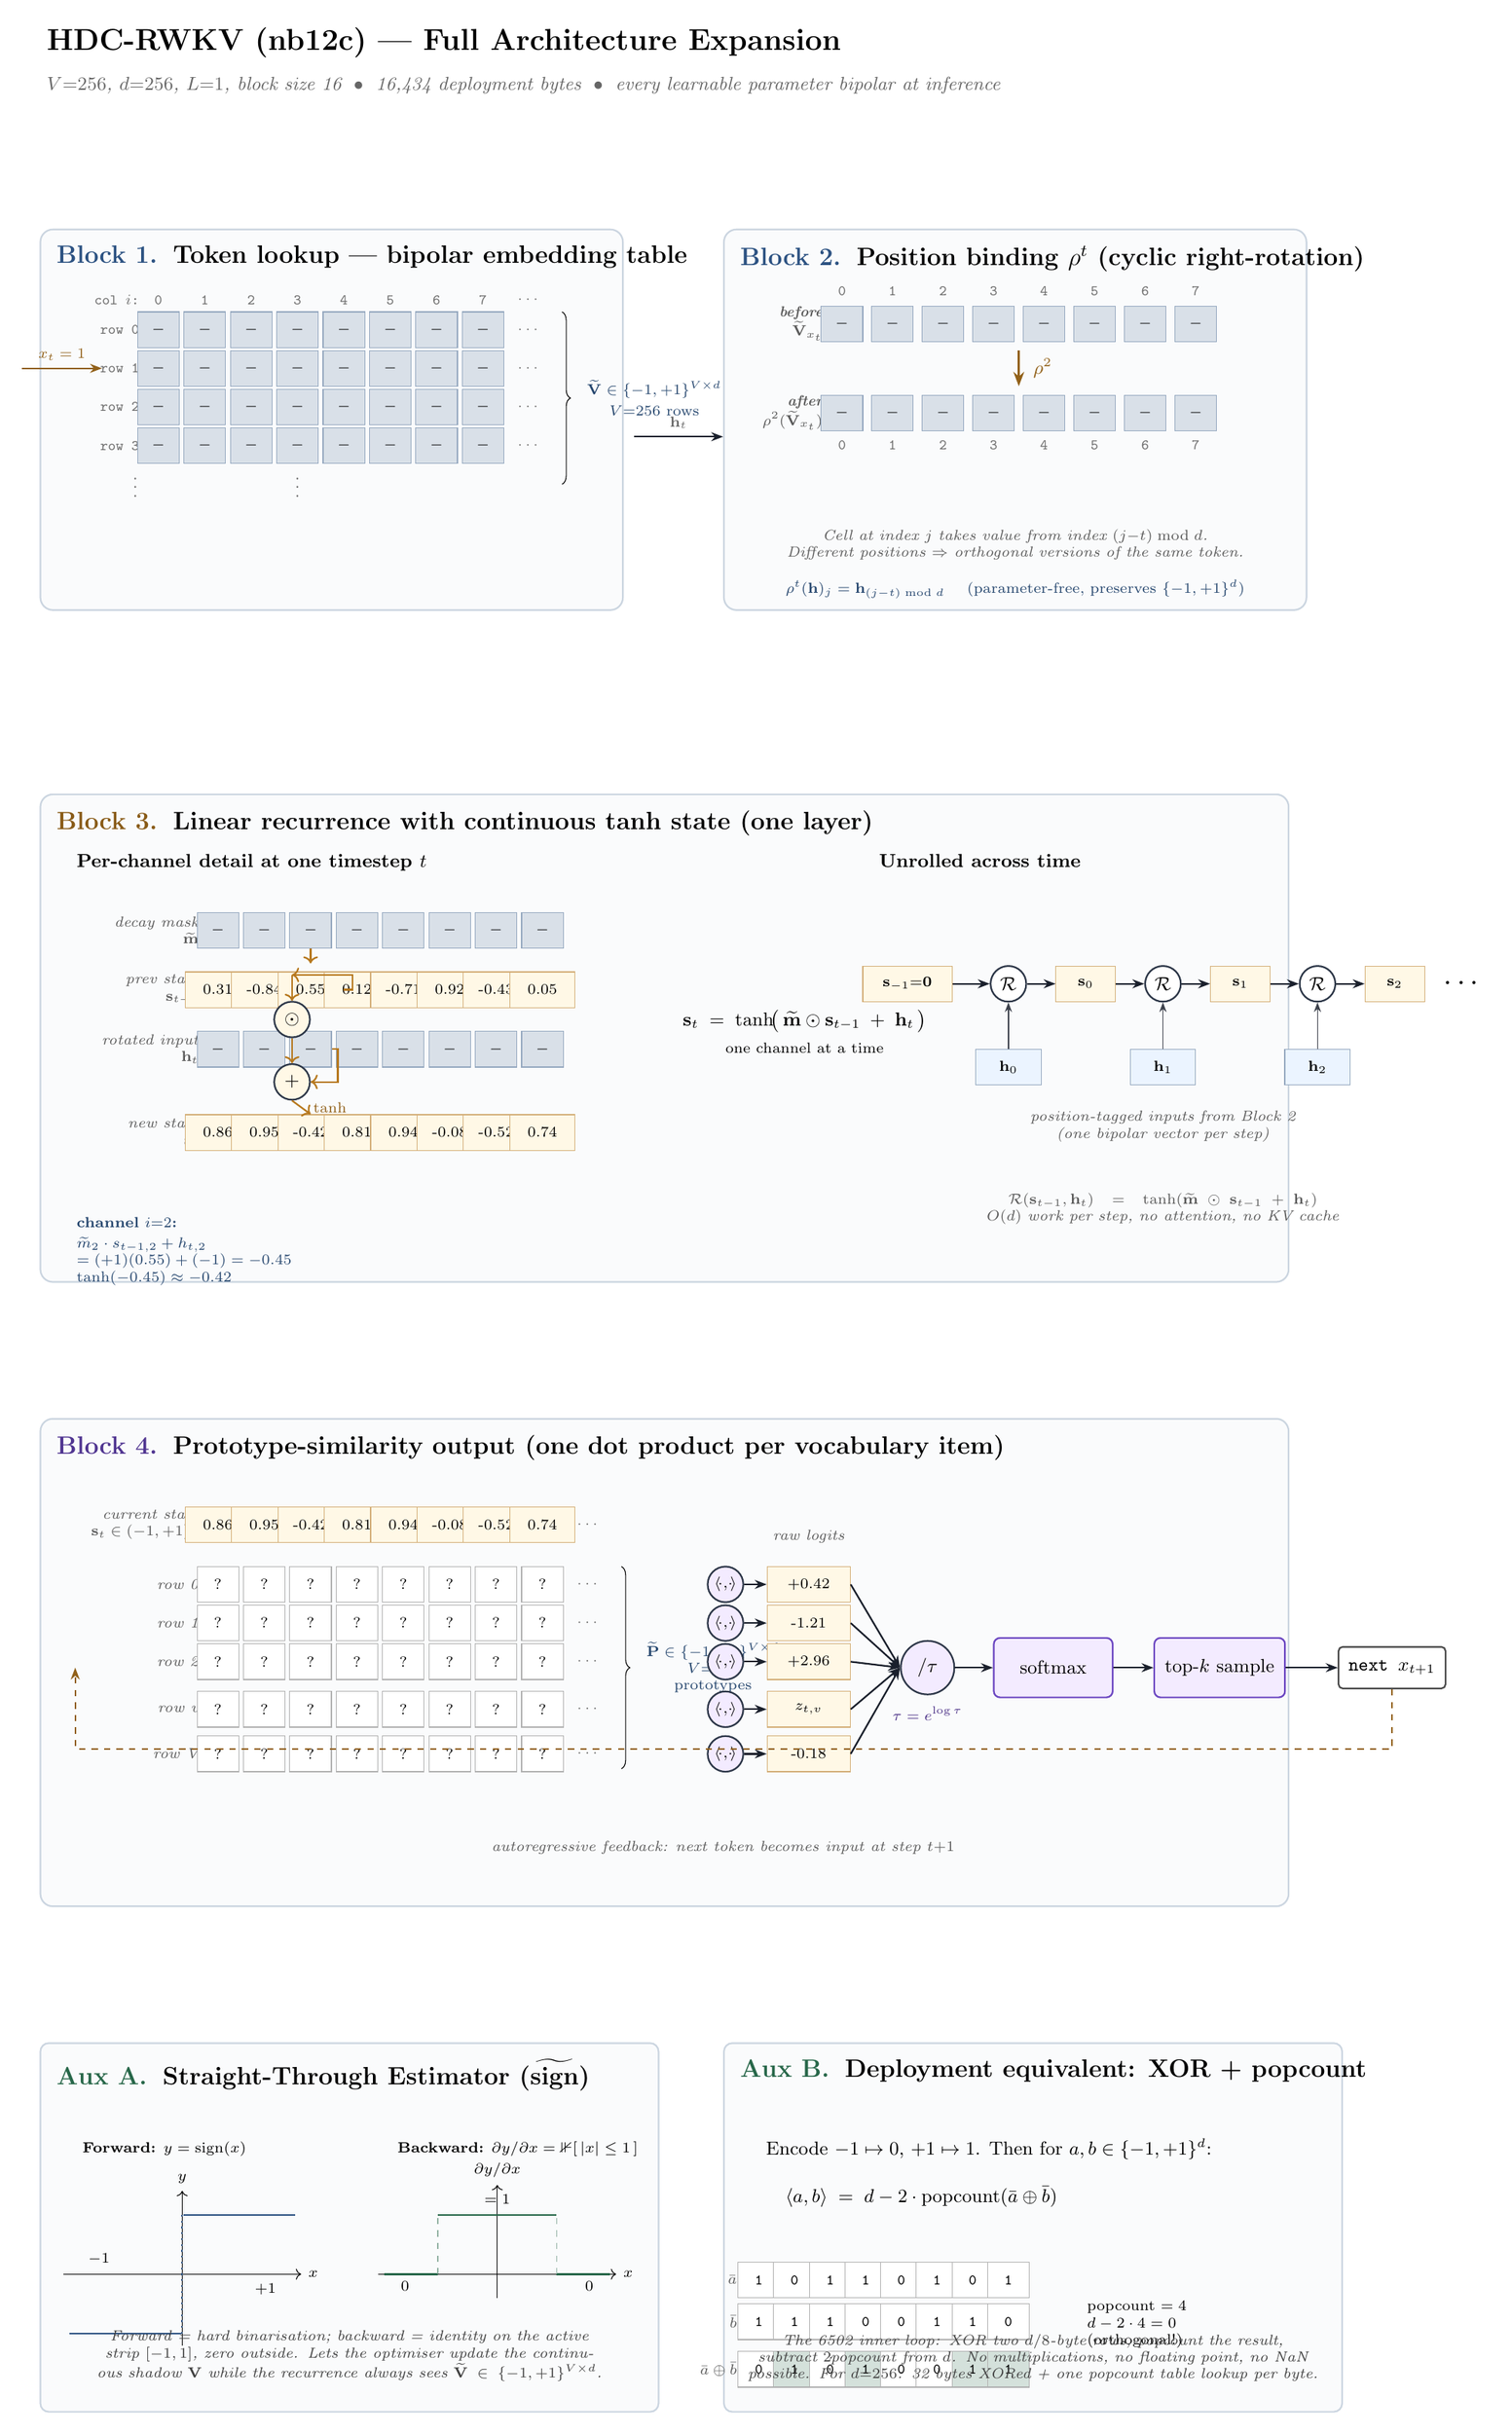
\begin{tikzpicture}

% =====================================================================
% TITLE
% =====================================================================
\node[font=\Large\bfseries, anchor=north west] (title) at (0,0)
  {HDC-RWKV (nb12c) --- Full Architecture Expansion};
\node[below=2pt of title.south west, font=\small\itshape, text=black!60,
      anchor=north west]
  {$V{=}256$, $d{=}256$, $L{=}1$, block size 16 \;$\bullet$\;
   16{,}434 deployment bytes \;$\bullet$\;
   every learnable parameter bipolar at inference};

% =====================================================================
% BLOCK 1 — TOKEN LOOKUP
% =====================================================================
\begin{scope}[shift={(0,-3.5)}]
  \node[block, minimum width=98mm, minimum height=64mm,
        anchor=north west] (B1) at (0,0) {};
  \node[blockTitle] at (B1.north west)
    {\textcolor{cBipolar}{Block 1.}\;\;Token lookup --- bipolar embedding table};

  % column index header
  \begin{scope}[shift={(2.0,-1.2)}]
    \node[idx, anchor=east] at (-0.2, 0) {col $i$:};
    \foreach \j in {0,1,2,3,4,5,6,7}
      \node[idx] at (\j*0.78, 0) {\j};
    \node[idx] at (8*0.78, 0) {$\cdots$};
  \end{scope}

  % rows
  \begin{scope}[shift={(2.0,-1.7)}]
    \foreach \row/\y/\pat in {0/0/{+,-,+,-,+,-,+,-},
                              1/-0.65/{-,+,-,+,-,+,-,+},
                              2/-1.30/{+,+,-,-,+,+,-,-},
                              3/-1.95/{+,-,-,+,+,+,-,-}} {
      \node[idx, anchor=east] at (-0.2, \y) {row \row};
      \foreach \v [count=\i from 0] in \pat {
        \ifx\v+
          \node[cellPos] (r\row_\i) at (\i*0.78, \y) {$+$};
        \else
          \node[cellNeg] (r\row_\i) at (\i*0.78, \y) {$-$};
        \fi
      }
      \node[idx] at (8*0.78, \y) {$\cdots$};
    }
    \node[idx, anchor=east] at (-0.2, -2.55) {$\vdots$};
    \node[idx] at (3*0.78, -2.55) {$\vdots$};

    % brace + matrix label on the far right
    \draw[decorate,decoration={brace,amplitude=4pt}]
      (8*0.78 + 0.55, 0.3) -- (8*0.78 + 0.55, -2.6);
    \node[matlbl, anchor=west] at (8*0.78 + 0.85, -1.15)
      {$\widetilde\bV \in \bipset^{V\times d}$\\[2pt] $V{=}256$ rows};

    % index pointer into row 1
    \draw[-{Stealth[length=2mm]}, thick, cCont!80!black]
      (-2.3, -0.65) -- (-0.95, -0.65)
      node[lbl, midway, above=0pt, text=cCont!80!black] {$x_t = 1$};
  \end{scope}
\end{scope}

% =====================================================================
% BLOCK 2 — POSITION BINDING ρ^t
% =====================================================================
\begin{scope}[shift={(11.5,-3.5)}]
  \node[block, minimum width=98mm, minimum height=64mm,
        anchor=north west] (B2) at (0,0) {};
  \node[blockTitle] at (B2.north west)
    {\textcolor{cBipolar}{Block 2.}\;\;Position binding $\rho^{t}$ (cyclic right-rotation)};

  % before row
  \begin{scope}[shift={(2.0,-1.6)}]
    \node[lbl, anchor=east, align=right] at (-0.2, 0)
      {\textbf{before}\\$\widetilde\bV_{x_t}$};
    \foreach \v [count=\i from 0] in {-,-,+,+,-,+,-,+} {
      \ifx\v+
        \node[cellPos] (in\i) at (\i*0.85, 0) {$+$};
      \else
        \node[cellNeg] (in\i) at (\i*0.85, 0) {$-$};
      \fi
      \node[idx, above=1pt of in\i] {\i};
    }

    % rotation arrow
    \draw[-{Stealth[length=2.4mm]}, very thick, cCont!80!black]
      (3.5*0.85, -0.45) -- (3.5*0.85, -1.05)
      node[midway, right=3pt, font=\small\bfseries, text=cCont!80!black] {$\rho^{2}$};

    % after row (rotation by 2 of pattern above)
    \node[lbl, anchor=east, align=right] at (-0.2, -1.5)
      {\textbf{after}\\$\rho^{2}(\widetilde\bV_{x_t})$};
    \foreach \v [count=\j from 0] in {-,+,-,-,+,+,-,+} {
      \ifx\v+
        \node[cellPos] (out\j) at (\j*0.85, -1.5) {$+$};
      \else
        \node[cellNeg] (out\j) at (\j*0.85, -1.5) {$-$};
      \fi
      \node[idx, below=1pt of out\j] {\j};
    }
  \end{scope}

  % caption + formula
  \node[lbl, align=center, text width=84mm, anchor=north]
    at ($(B2.south)+(0,1.5)$)
    {Cell at index $j$ takes value from index $(j{-}t)\bmod d$.\\
     Different positions $\Rightarrow$ orthogonal versions of the same token.};
  \node[matlbl, anchor=north] at ($(B2.south)+(0,0.65)$)
    {$\rho^{t}(\bh)_j = \bh_{(j-t)\bmod d}$ \quad
     (parameter-free, preserves $\bipset^{d}$)};
\end{scope}

% Arrow B1 -> B2
\draw[flow, thick] (10,-7) -- (11.5,-7)
  node[lbl, midway, above, text=black!60] {$\bh_t$};

% =====================================================================
% BLOCK 3 — RECURRENCE
% =====================================================================
\begin{scope}[shift={(0,-13)}]
  \node[block, minimum width=210mm, minimum height=82mm,
        anchor=north west] (B3) at (0,0) {};
  \node[blockTitle] at (B3.north west)
    {\textcolor{cCont!75!black}{Block 3.}\;\;Linear recurrence with continuous tanh state (one layer)};

  % ---- LEFT: per-channel detail ----
  \node[font=\small\bfseries, anchor=north west] at ($(B3.north west)+(0.5,-0.9)$)
     {Per-channel detail at one timestep $t$};

  \begin{scope}[shift={(3.0,-2.3)}]
    % decay_mask row
    \node[lbl, anchor=east, align=right] at (-0.2, 0)
       {decay mask\\$\widetilde\bm$};
    \foreach \v [count=\i from 0] in {+,-,+,+,-,+,-,-} {
      \ifx\v+
        \node[cellPos] (m\i) at (\i*0.78, 0) {$+$};
      \else
        \node[cellNeg] (m\i) at (\i*0.78, 0) {$-$};
      \fi
    }

    % prev state
    \node[lbl, anchor=east, align=right] at (-0.2, -1.0)
       {prev state\\$\bs_{t-1}$};
    \foreach \v [count=\i from 0] in {0.31,-0.84,0.55,0.12,-0.71,0.92,-0.43,0.05} {
      \node[cellCont] (s\i) at (\i*0.78, -1.0) {\v};
    }

    % rotated input h_t
    \node[lbl, anchor=east, align=right] at (-0.2, -2.0)
       {rotated input\\$\bh_t$};
    \foreach \v [count=\i from 0] in {+,+,-,+,+,-,-,+} {
      \ifx\v+
        \node[cellPos] (h\i) at (\i*0.78, -2.0) {$+$};
      \else
        \node[cellNeg] (h\i) at (\i*0.78, -2.0) {$-$};
      \fi
    }

    % new state s_t
    \node[lbl, anchor=east, align=right] at (-0.2, -3.4)
       {new state\\$\bs_t$};
    \foreach \v [count=\i from 0] in {0.86,0.95,-0.42,0.81,0.94,-0.08,-0.52,0.74} {
      \node[cellCont] (sn\i) at (\i*0.78, -3.4) {\v};
    }

    % wiring for channel i=2
    \draw[->, thick, cCont] (m2.south) -- ++(0,-0.25);
    \draw[->, thick, cCont] (s2.east) -- ++(0.15,0) |- (1.6*0.78, -0.75);
    \node[op, fill=cContLite] (mul2) at (1.6*0.78, -1.5) {$\odot$};
    \draw[->, thick, cCont] (1.6*0.78, -0.75) -- (mul2.north);
    \node[op, fill=cContLite] (add2) at (1.6*0.78, -2.55) {$+$};
    \draw[->, thick, cCont] (mul2.south) -- (add2.north);
    \draw[->, thick, cCont] (h2.east) -- ++(0.1,0) |- (add2.east);
    \draw[->, thick, cCont] (add2.south) -- (sn2.north)
      node[midway, right=2pt, lbl, text=cCont!80!black] {$\tanh$};
  \end{scope}

  % channel-2 worked example (placed in clear space below right of the cells)
  \node[matlbl, align=left, anchor=north west,
        text width=42mm]
        at ($(B3.north west)+(0.5,-7.0)$)
    {\textbf{channel $i{=}2$:}\\[2pt]
     $\widetilde m_2 \cdot s_{t-1,2} + h_{t,2}$\\
     $= (+1)(0.55) + (-1) = -0.45$\\
     $\tanh(-0.45) \approx -0.42$};

  % equation on the right of the per-channel block
  \node[eqn, align=center, anchor=west]
        at ($(B3.north west)+(10.7,-4.0)$)
     {$\bs_t \;=\; \tanh\!\bigl(\,\widetilde\bm \odot \bs_{t-1} \;+\; \bh_t\,\bigr)$\\[2pt]
      \scriptsize one channel at a time};

  % ---- RIGHT: time-unrolled ----
  \node[font=\small\bfseries, anchor=north west]
        at ($(B3.north west)+(14.0,-0.9)$) {Unrolled across time};

  \begin{scope}[shift={(14.6,-3.2)}]
    \node[cellCont, minimum width=15mm] (st0) at (0,   0) {$\bs_{-1}{=}\mathbf{0}$};
    \node[op] (rec0) at (1.7, 0) {$\mathcal{R}$};
    \node[cellCont, minimum width=10mm] (st1) at (3.0, 0) {$\bs_0$};
    \node[op] (rec1) at (4.3, 0) {$\mathcal{R}$};
    \node[cellCont, minimum width=10mm] (st2) at (5.6, 0) {$\bs_1$};
    \node[op] (rec2) at (6.9, 0) {$\mathcal{R}$};
    \node[cellCont, minimum width=10mm] (st3) at (8.2, 0) {$\bs_2$};
    \node[font=\Large, anchor=west] at (8.9, 0) {$\cdots$};
    \foreach \a/\b in {st0/rec0, rec0/st1, st1/rec1, rec1/st2, st2/rec2, rec2/st3}
      \draw[flow] (\a) -- (\b);

    % per-step inputs (placed 1.4cm below each \mathcal{R} box)
    \foreach \i/\rname in {0/rec0, 1/rec1, 2/rec2} {
      \node[cellPos, minimum width=11mm] (hin\i)
        at ([yshift=-1.4cm]\rname) {$\bh_{\i}$};
      \draw[flowSm] (hin\i.north) -- (\rname.south);
    }
    \node[lbl, align=center, text width=70mm] at (4.3, -2.4)
       {position-tagged inputs from Block 2\\(one bipolar vector per step)};

    \node[lbl, align=center, text width=85mm, anchor=north] at (4.3, -3.4)
       {$\mathcal{R}(\bs_{t-1}, \bh_t) = \tanh(\widetilde\bm \odot \bs_{t-1} + \bh_t)$\\
        $O(d)$ work per step, no attention, no KV cache};
  \end{scope}
\end{scope}

% =====================================================================
% BLOCK 4 — PROTOTYPE OUTPUT
% =====================================================================
\begin{scope}[shift={(0,-23.5)}]
  \node[block, minimum width=210mm, minimum height=82mm,
        anchor=north west] (B4) at (0,0) {};
  \node[blockTitle] at (B4.north west)
    {\textcolor{cSampler!75!black}{Block 4.}\;\;Prototype-similarity output (one dot product per vocabulary item)};

  \begin{scope}[shift={(3.0,-1.8)}]
    % current state s_t (header row)
    \node[lbl, anchor=east, align=right] at (-0.2, 0)
      {current state\\$\bs_t \in (-1,+1)^{d}$};
    \foreach \v [count=\i from 0] in {0.86,0.95,-0.42,0.81,0.94,-0.08,-0.52,0.74} {
      \node[cellCont] (ss\i) at (\i*0.78, 0) {\v};
    }
    \node[idx] at (8*0.78, 0) {$\cdots$};

    % prototype rows
    \foreach \row/\y/\pat in {0/-1.0/{+,+,-,-,+,+,-,-},
                              1/-1.65/{-,+,+,-,-,+,+,-},
                              2/-2.30/{+,-,+,-,+,-,+,-},
                              v/-3.10/{?,?,?,?,?,?,?,?},
                              V/-3.85/{-,-,+,+,-,+,-,+}} {
      \node[lbl, anchor=east] at (-0.2, \y) {row \row};
      \foreach \v [count=\i from 0] in \pat {
        \ifx\v+
          \node[cellPos] (p\row_\i) at (\i*0.78, \y) {$+$};
        \else\ifx\v-
          \node[cellNeg] (p\row_\i) at (\i*0.78, \y) {$-$};
        \else
          \node[cellPlain] (p\row_\i) at (\i*0.78, \y) {?};
        \fi\fi
      }
      \node[idx] at (8*0.78, \y) {$\cdots$};
    }

    % brace on prototype matrix
    \draw[decorate, decoration={brace, amplitude=4pt}]
      (8*0.78 + 0.55, -0.7) -- (8*0.78 + 0.55, -4.1);
    \node[matlbl, anchor=west] at (8*0.78 + 0.85, -2.4)
      {$\widetilde\bP \in \bipset^{V\times d}$\\$V{=}256$\\prototypes};

    % dot products
    \foreach \row/\y/\val in {0/-1.0/{+0.42},
                              1/-1.65/{-1.21},
                              2/-2.30/{+2.96},
                              v/-3.10/{$z_{t,v}$},
                              V/-3.85/{-0.18}} {
      \node[op, fill=cSamplerLite] (dot\row) at (8*0.78 + 2.3, \y)
        {\scriptsize$\langle\!\cdot,\!\cdot\!\rangle$};
      \node[cellCont, minimum width=14mm] (lg\row) at (8*0.78 + 3.7, \y) {\val};
      \draw[flow] (dot\row) -- (lg\row);
    }
    \node[lbl] at (8*0.78 + 3.7, -0.2) {raw logits};

    % temperature divide
    \node[op, fill=cSamplerLite, minimum size=9mm] (divT)
        at (8*0.78 + 5.7, -2.4) {$/\tau$};
    \node[lbl, below=2pt of divT, text=cSampler!70!black] {$\tau = e^{\log\tau}$};
    \foreach \row/\y in {0/-1.0, 1/-1.65, 2/-2.30, v/-3.10, V/-3.85}
      \draw[flow] (lg\row.east) -- (divT.west);

    % softmax + top-k
    \node[draw=cSampler, fill=cSamplerLite, thick, rounded corners=3pt,
          minimum width=20mm, minimum height=10mm, font=\small, anchor=west]
          (sm) at (8*0.78 + 6.8, -2.4) {softmax};
    \draw[flow] (divT) -- (sm);
    \node[draw=cSampler, fill=cSamplerLite, thick, rounded corners=3pt,
          minimum width=22mm, minimum height=10mm, font=\small, anchor=west]
          (tk) at (8*0.78 + 9.5, -2.4) {top-$k$ sample};
    \draw[flow] (sm) -- (tk);
    \node[draw=black!70, thick, rounded corners=2pt, minimum width=18mm,
          minimum height=7mm, font=\small\ttfamily, anchor=west]
          (nxt) at (8*0.78 + 12.6, -2.4) {next $x_{t+1}$};
    \draw[flow] (tk) -- (nxt);

    % autoregressive feedback
    \draw[recur] (nxt.south) -- ++(0,-1.0) -| (-2.4, -2.4);
    \node[lbl, align=center, anchor=north] at (8.5, -5.2)
      {autoregressive feedback: next token becomes input at step $t{+}1$};
  \end{scope}
\end{scope}

% =====================================================================
% AUX A — STE forward/backward
% =====================================================================
\begin{scope}[shift={(0,-34)}]
  \node[panel, minimum width=104mm, minimum height=62mm,
        anchor=north west] (AA) at (0,0) {};
  \node[blockTitle] at (AA.north west)
    {\textcolor{cAux}{Aux A.}\;\;Straight-Through Estimator ($\widetilde{\text{sign}}$)};

  \begin{scope}[shift={(0.6,-1.8)}]
    % header lines first so they don't overlap plots
    \node[font=\scriptsize, anchor=west] at (0,   0) {\textbf{Forward:} $y = \mathrm{sign}(x)$};
    \node[font=\scriptsize, anchor=west] at (5.3, 0) {\textbf{Backward:} $\partial y/\partial x = \mathbb{1}[\,|x|\le 1\,]$};

    % forward plot
    \begin{scope}[shift={(1.8,-2.1)}]
      \draw[->] (-2.0,0) -- (2.0,0) node[right, font=\scriptsize] {$x$};
      \draw[->] (0,-1.2) -- (0,1.4) node[above, font=\scriptsize] {$y$};
      \draw[thick, cBipolar] (-1.9,-1) -- (-0.02,-1);
      \draw[thick, cBipolar] (0.02, 1) -- ( 1.9, 1);
      \draw[thick, cBipolar, dotted] (0,-1) -- (0,1);
      \node[font=\scriptsize] at (1.4,-0.25) {$+1$};
      \node[font=\scriptsize] at (-1.4,0.25) {$-1$};
    \end{scope}

    % backward plot
    \begin{scope}[shift={(7.1,-2.1)}]
      \draw[->] (-2.0,0) -- (2.0,0) node[right, font=\scriptsize] {$x$};
      \draw[->] (0,-0.4) -- (0,1.5) node[above, font=\scriptsize] {$\partial y/\partial x$};
      \draw[thick, cAux] (-1.9,0) -- (-1.0,0);
      \draw[thick, cAux] (-1.0,1) -- (1.0, 1);
      \draw[thick, cAux] (1.0, 0) -- (1.9, 0);
      \draw[dashed, cAux!50] (-1.0,0) -- (-1.0,1);
      \draw[dashed, cAux!50] ( 1.0,0) -- ( 1.0,1);
      \node[font=\scriptsize, anchor=south] at (0,1.05) {$=1$};
      \node[font=\scriptsize] at (-1.55,-0.2) {$0$};
      \node[font=\scriptsize] at ( 1.55,-0.2) {$0$};
    \end{scope}
  \end{scope}

  \node[lbl, align=center, text width=96mm, anchor=south,
        text=black!75]
    at ($(AA.south)+(0,0.4)$)
    {Forward = hard binarisation; backward = identity on the active strip
     $[-1,1]$, zero outside. Lets the optimiser update the continuous
     shadow $\bV$ while the recurrence always sees
     $\widetilde\bV \in \bipset^{V\times d}$.};
\end{scope}

% =====================================================================
% AUX B — XOR + popcount
% =====================================================================
\begin{scope}[shift={(11.5,-34)}]
  \node[panel, minimum width=104mm, minimum height=62mm,
        anchor=north west] (AB) at (0,0) {};
  \node[blockTitle] at (AB.north west)
    {\textcolor{cAux}{Aux B.}\;\;Deployment equivalent: XOR + popcount};

  \begin{scope}[shift={(0.6,-1.8)}]
    \node[font=\small, anchor=west] at (0, 0)
      {Encode $-1\mapsto 0$, $+1\mapsto 1$. Then for $a,b\in\bipset^d$:};
    \node[font=\small, anchor=west] at (0, -0.8)
      {$\quad\langle a,b\rangle \;=\; d - 2\cdot\mathrm{popcount}(\bar a \oplus \bar b)$};

    % toy example
    \begin{scope}[shift={(0,-2.2)}]
      \node[lbl, anchor=east] at (-0.15, 0) {$\bar a$:};
      \foreach \v [count=\i from 0] in {1,0,1,1,0,1,0,1}
        \node[cellPlain, font=\scriptsize\ttfamily] at (\i*0.6, 0) {\v};

      \node[lbl, anchor=east] at (-0.15, -0.7) {$\bar b$:};
      \foreach \v [count=\i from 0] in {1,1,1,0,0,1,1,0}
        \node[cellPlain, font=\scriptsize\ttfamily] at (\i*0.6, -0.7) {\v};

      \node[lbl, anchor=east] at (-0.15, -1.5) {$\bar a\oplus\bar b$:};
      \foreach \v [count=\i from 0] in {0,1,0,1,0,0,1,1} {
        \ifnum\v=1
          \node[cellPlain, fill=cAux!20, font=\scriptsize\ttfamily] at (\i*0.6, -1.5) {\v};
        \else
          \node[cellPlain, font=\scriptsize\ttfamily] at (\i*0.6, -1.5) {\v};
        \fi
      }

      \node[font=\scriptsize, anchor=west, align=left] at (5.4, -0.75)
        {popcount $= 4$\\$d - 2\cdot 4 = 0$\\(orthogonal!)};
    \end{scope}
  \end{scope}

  \node[lbl, align=center, text width=96mm, anchor=south, text=black!75]
    at ($(AB.south)+(0,0.4)$)
    {The 6502 inner loop: XOR two $d/8$-byte rows, popcount the result,
     subtract $2\!\cdot\!$popcount from $d$. No multiplications, no floating
     point, no NaN possible. For $d{=}256$: 32 bytes XORed + one popcount
     table lookup per byte.};
\end{scope}

\end{tikzpicture}
\end{document}
